% !TEX root = Calli.tex
% Einstellungen
\documentclass[10pt, DIV12, a4paper]{scrartcl}
\usepackage[utf8]{inputenc}
\usepackage[T1]{fontenc}
\usepackage{lmodern}
\usepackage[ngerman]{babel}
\usepackage{amsmath}
\usepackage{nicefrac}
\usepackage{graphicx, wrapfig, float}
\usepackage[onehalfspacing]{setspace}
\usepackage{paralist}  % \begin{compactitem}
\usepackage{listings, color}
\usepackage[parfill]{parskip}
\usepackage{setspace}
\usepackage{tabularx}
\usepackage{booktabs}
\usepackage{multirow}
\usepackage{multicol}
\usepackage{pdfpages}
\usepackage{lscape}

\onehalfspacing
\setcounter{tocdepth}{2} % Tiefe Inhaltsverzeichnis
\numberwithin{figure}{section}
\setkomafont{sectioning}{\normalcolor\bfseries}

% -------------------
% Quelltextanzeige
\usepackage{listings, color}
\lstset{language= python}

\newcommand{\lstfontfamily}{\ttfamily}
%\newcommand{\lstfontfamily}{\sffamily} % Adapt to schneider
\newcommand{\textlst}[1]{\texttt{#1}}
\newcommand{\mathlst}[1]{\mathtt{#1}}
\lstdefinestyle{tiny}{basicstyle=\tiny\lstfontfamily}
\lstdefinestyle{scriptsize}{basicstyle=\scriptsize\lstfontfamily}
\lstdefinestyle{footnotesize}{basicstyle=\footnotesize\lstfontfamily}
\lstdefinestyle{small}{basicstyle=\small\lstfontfamily}
\lstdefinestyle{normalsize}{basicstyle=\normalsize\lstfontfamily}
\lstdefinestyle{large}{basicstyle=\lstfontfamily}

\lstdefinestyle{monitor}{morekeywords={monitor, export}}
\lstdefinestyle{ConcPascal}{language=Pascal,style=monitor}
\newcommand{\mathcodefont}[1]{\mathtt{#1}}
\newcommand{\codefont}[1]{{\lstfontfamily #1}}
\newlength{\lstframexleftmargin}
\setlength{\lstframexleftmargin}{1mm}

\definecolor{darkviolet}{rgb}{0.5,0,0.4}
\definecolor{darkgreen}{rgb}{0,0.4,0.2}
\definecolor{darkblue}{rgb}{0.1,0.1,0.9}
\definecolor{darkgrey}{rgb}{0.5,0.5,0.5}
\definecolor{lightblue}{rgb}{0.4,0.4,1}

\lstdefinestyle{eclipse}{
    basicstyle=\small\lstfontfamily,
    emphstyle=\color{red}\bfseries,
    keywordstyle=\color{darkviolet}\bfseries,
    commentstyle=\color{darkgreen},
    stringstyle=\color{darkblue},
    numberstyle=\color{darkgrey}\lstfontfamily,
    emphstyle=\color{red},
    % get also javadoc style comments
    morecomment=[s][\color{lightblue}]{/**}{*/},
    morekeywords={@start, @stop, @v, @about, @demo_translation, @demo_forward, @demo_sideways, @demo_stopWithDelay, uint8_t, uint16_t, int16_t, int8_t, byte},
   %columns=fullflexible, %spaceflexible, %flexible, fullflexible
%  escapeinside=`',
%  escapechar=@,
  showstringspaces=false,
  numbers=left
}

\definecolor{lstBg}{rgb}{0.98, 0.98, 0.98}
\definecolor{lstFrame}{rgb}{0.8, 0.8, 0.8}
\lstset{
    language = C,
    style=eclipse,
    tabsize=4,
    basicstyle = \ttfamily,
    title=\lstname,
    % numbers=none,
    backgroundcolor=\color{lstBg},
    rulecolor=\color{lstFrame},
    frame=lines,
    %captionpos=b,
    aboveskip=1\bigskipamount,%{1.5\baselineskip},
    showstringspaces=false,
    extendedchars=true,
    breaklines=false,
    literate=%
        {Ö}{{\"O}}1
        {Ä}{{\"A}}1
        {Ü}{{\"U}}1
        {ß}{{\ss}}1
        {ü}{{\"u}}1
        {ä}{{\"a}}1
        {ö}{{\"o}}1
}


\titlehead{
    \begin{tabular}{l p{9cm} c}
        & & 
\includegraphics[width=0.4\textwidth]{Abbildungen/W-HS} \\
        & & \textbf{Fachbereich Maschinenbau} \\

    \end{tabular}
    \vspace{1.5cm}}
\subject{Projektbericht\\Instustrielle Bildverarbeitung}

\title{Halli Galli - CV\vspace{1.5cm}}
\subtitle{Spielstandanalyse mit einer Webcam\vspace{3cm}}

\author{
    \begin{tabular}{rl}
        Manuel Fehmer & 200923513 \\
        Marlene Feldmann & 200825051 \\
    \end{tabular}\vspace{0.3cm}
}

\begin{document}
\begin{titlepage}
\maketitle
\pagenumbering{gobble}
\end{titlepage}
\tableofcontents
\pagenumbering{arabic}
\newpage

% !TEX root = Calli.tex
% Kapitelvorlage

\section{Einleitung}
\label{sec:Einleitung}

Die Anforderungen an die Qualität industriell gefertigter Endprodukte werden immer höher. Um die Kosten der Endkontrolle möglichst gering zu halten, wird eine fehlerresistente und automatisierte Prüfung angestrebt. In vielen Fällen werden dazu Industriekameras eingesetzt. Mit einer angepassten Beleuchtung, der entsprechenden Ausrichtung und einer ausgereiften Software ersetzen sie mittlerweile viele manuelle Kontrollen. Insbesondere zur Farb- und Formerkennung sind sie gut geeignet.

Das bearbeitete Thema hat zum Gegenstand eine Farb- und Formerkennung mit einer Kamera zu realisieren. Grundlage ist das Reaktionsspiel Halli Galli\footnote{\cite{HalliGalli}}. 

\begin{figure}[H]
    \centering
    \includegraphics[width=7cm]{Abbildungen/cover}
    \caption[Cocer]{Halli Galli - Spielcover}
    \label{fig:Cover}
\end{figure}

\subsection{Halli Galli}

Halli Galli ist ein Reaktionskartenspiel für Kinder. Obwohl das Spielprinzip sehr einfach ist, ist es aufgrund der hohen Spielgeschwindigkeit, der geforderten Konzentrationsfähigkeit sowie der Stressresistenz auch bei vielen Erwachsenen beliebt. 

\textbf{Ziel des Spiels}

Ziel ist es in den Besitz aller Spielkarten zu kommen. Ist dies nicht möglich, gewinnt der Spieler mit den meisten Karten. Hat ein Spieler alle Karten verloren, scheidet er aus. 



\begin{figure}[H]
    \centering
    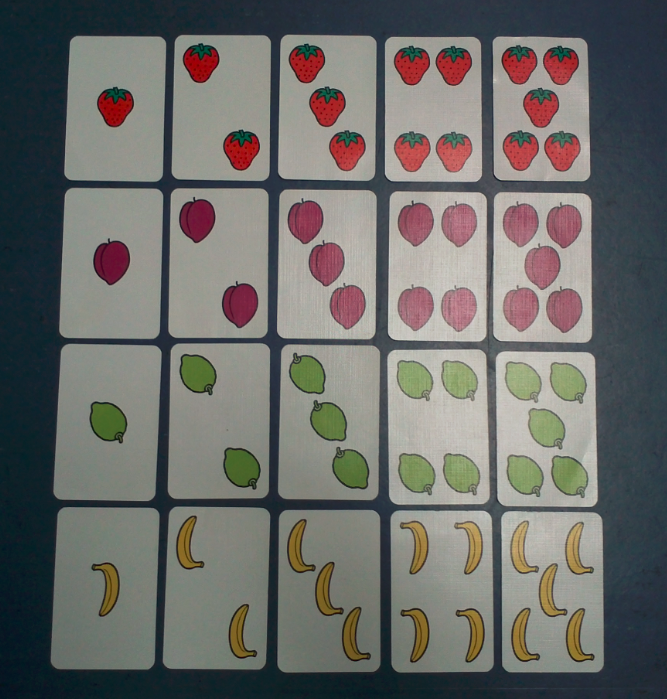
\includegraphics[width=8cm]{Abbildungen/Kartenset}
    \caption[Cocer]{Halli Galli - Kartenset}
    \label{fig:Kartenset}
\end{figure}
\textbf{Spielanleitung}

Alle 56 Fruchtkarten des Kartensets, siehe Abbildung \ref{fig:Kartenset}, werden gleichmäßig an die Mitspieler verteilt. Reihum decken die Spieler die Karten von ihrem Zugstapel auf und legen sie vor sich auf einen separaten Ablagestabel ab. Nach jedem Zug müssen die Früchte auf den offenen Karten gezählt werden. Entspricht die Anzahl einer Sorte genau fünf, so darf auf die Glocke geschlagen werden. Der erste der die Glocke betätigt darf alle offenen Karten einsammeln und unter seinen Zugstapel leben. Reagiert ein Spieler falsch, so muss er jedem Mitspieler eine Karte von seinem Zugstapel geben. 

\subsection{Aufgabenstellung}


Ziel der Projektarbeit ist es mit einer Kamera ein simuliertes Halli Galli Spielfeld von vier Spielern von oben zu filmen. Die Kamera erkennt die Früchte auf den Karten und gibt über eine Bildschirmausgabe an, wenn fünf Früchte einer Sorte erkannt wurden. Abgebildet werden Limonen, Erdbeeren, Pflaumen und Bananen. Schwierigkeiten entstehen durch die zum Teil sehr ähnlichen Farben und Formen der Früchte.

\subsection{Aufbau}
\label{sub:Aufbau}

Abbildung~\ref{fig:Anlage} zeigt den benutzten Aufbau zur Erfassung des Spielstandes. Eine Webcam mit USB~-~Schnittstelle wird mit Hilfe eines Aluprofils 40 cm über dem Spielaufbau positioniert.

%Abbildung Aufbau / Kamera
\begin{figure}[]
    \centering
    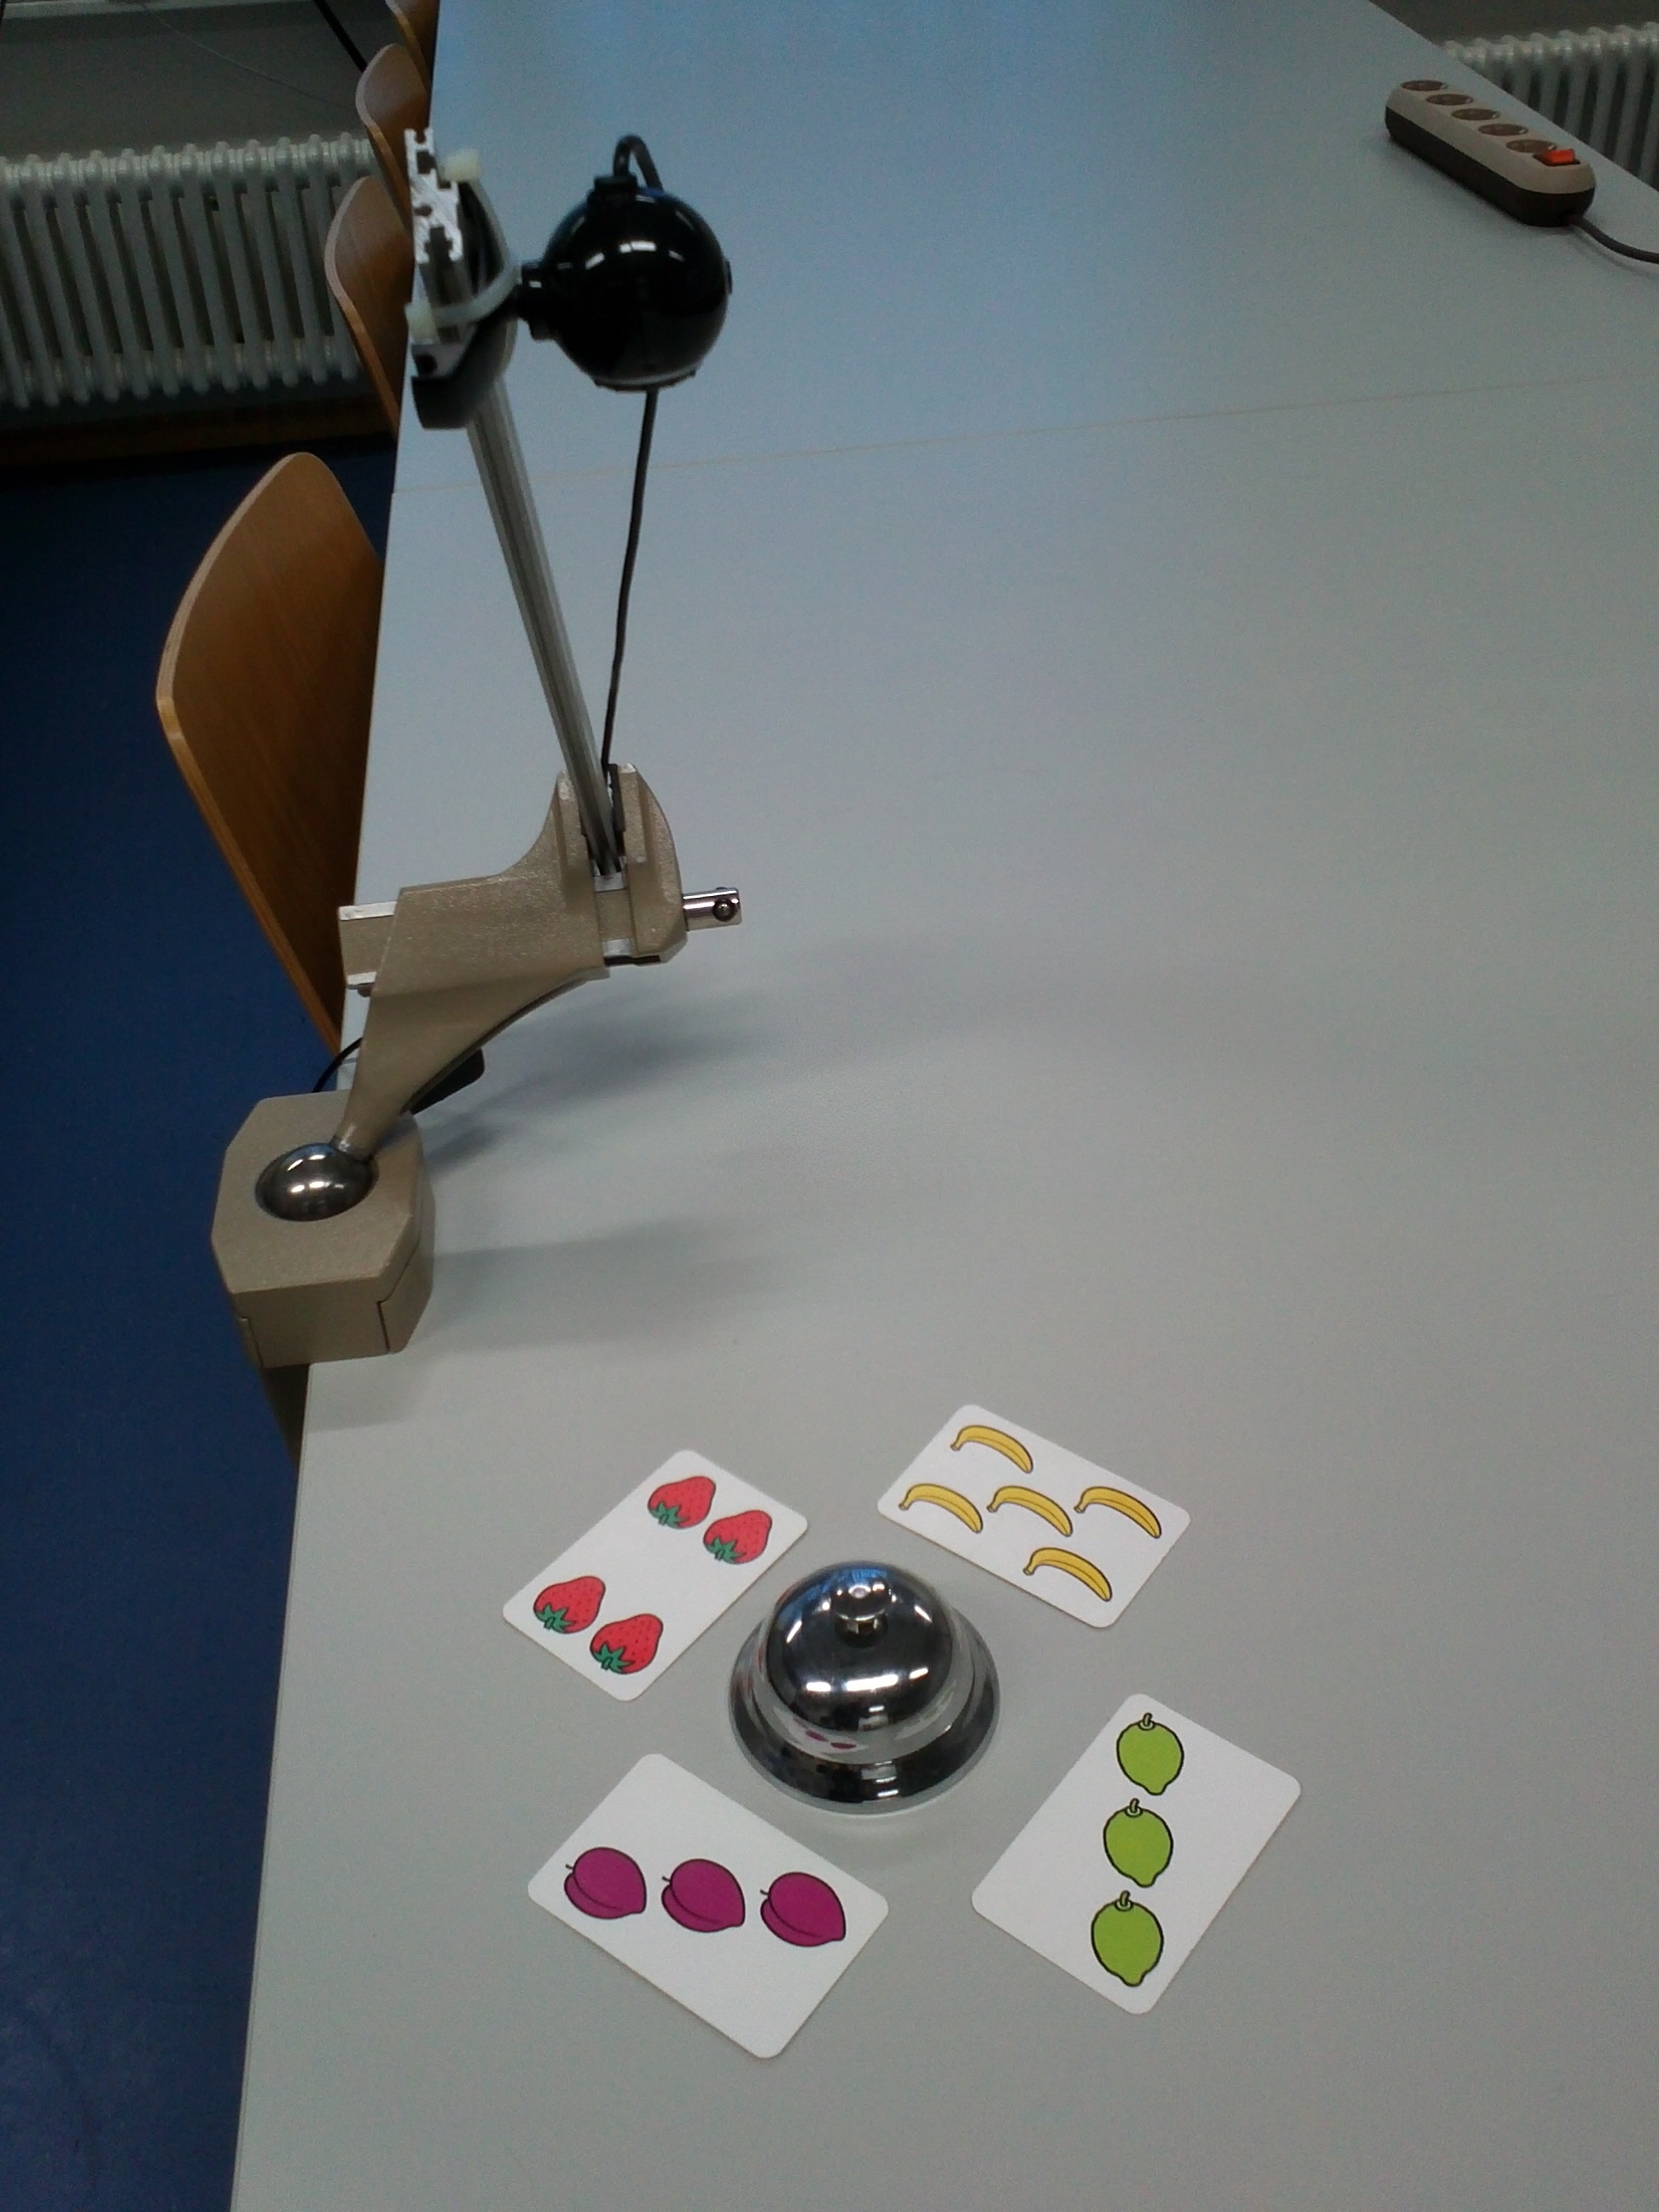
\includegraphics[width=7cm]{Abbildungen/KameraAufbau}
    \caption[Anlage]{Anlagenaufbau}
    \label{fig:Anlage}
\end{figure}

Der Spielaufbau entspricht dem original Halli Galli Aufbau mit vier Mitspielern. Abbildung~\ref{fig:Spielaufbau} zeigt die mittig positionierte Glocke, um die vier Ablagestabel der Spieler angeordnet sind.\\

%Abbildung Foto, wie die Karten liegen
\begin{figure}[h]
    \centering
    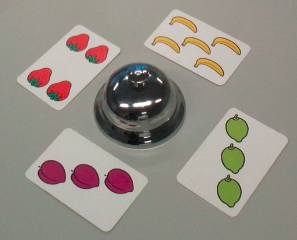
\includegraphics[width=6cm]{Abbildungen/Aufbau4}
    \caption[Spielaufbau]{Halli Galli - Spielaufbau mit vier Mitspielern}
    \label{fig:Spielaufbau}
\end{figure}


%hier sollen die vier Spielkarten (vier Früchte einzeln sein)

%\begin{center}
%\begin{tabular}{cccc}
  %
\includegraphics[width=3cm]{Abbildungen/Cover} & 
\includegraphics[width=3cm]{Abbildungen/Cover} & %
\includegraphics[width=3cm]{Abbildungen/Cover} & 
\includegraphics[width=3cm]{Abbildungen/Cover} \\ 
%\end{tabular}

%\end{center}





%1.) Theoretische Grundlagen (z.B. Messprinzip)

%2.) Genaue Beschreibung des Geräteaufbaus (Bilder)

%3.) Beschreibung der Halcon-Programmstruktur und die Funktionsweise der Programmblöcke

%4.) Gut dokumentierter Halcon-Code 

%) Ergebnisse 

%6.) Testbilder, um das Programm auch ohne Kamera testen zu können.

%Die Doku auf CD mit allen Bilder muss dem gedruckten Bericht beigelegt werden.

%BILDER:

%Jede Frucht einmal einzeln - Foto von der Karte

%Screenshot - von den schwarz / weiß Erkennung - inkl. Bild dazu 

%verschiedene Test - Bilder

%% !TEX root = Calli.tex

\section{Aufbau}
\label{sec:Kapitel}

Abbildung~\ref{fig:Anlage} zeigt den benutzten Aufbau zur Erfassung des Spielstandes. Eine Webcam mit USB~-~Schnittstelle wird mit Hilfe eines Aluprofils 40 cm über dem Spielaufbau positioniert.

%Abbildung Aufbau / Kamera
\begin{figure}[]
    \centering
    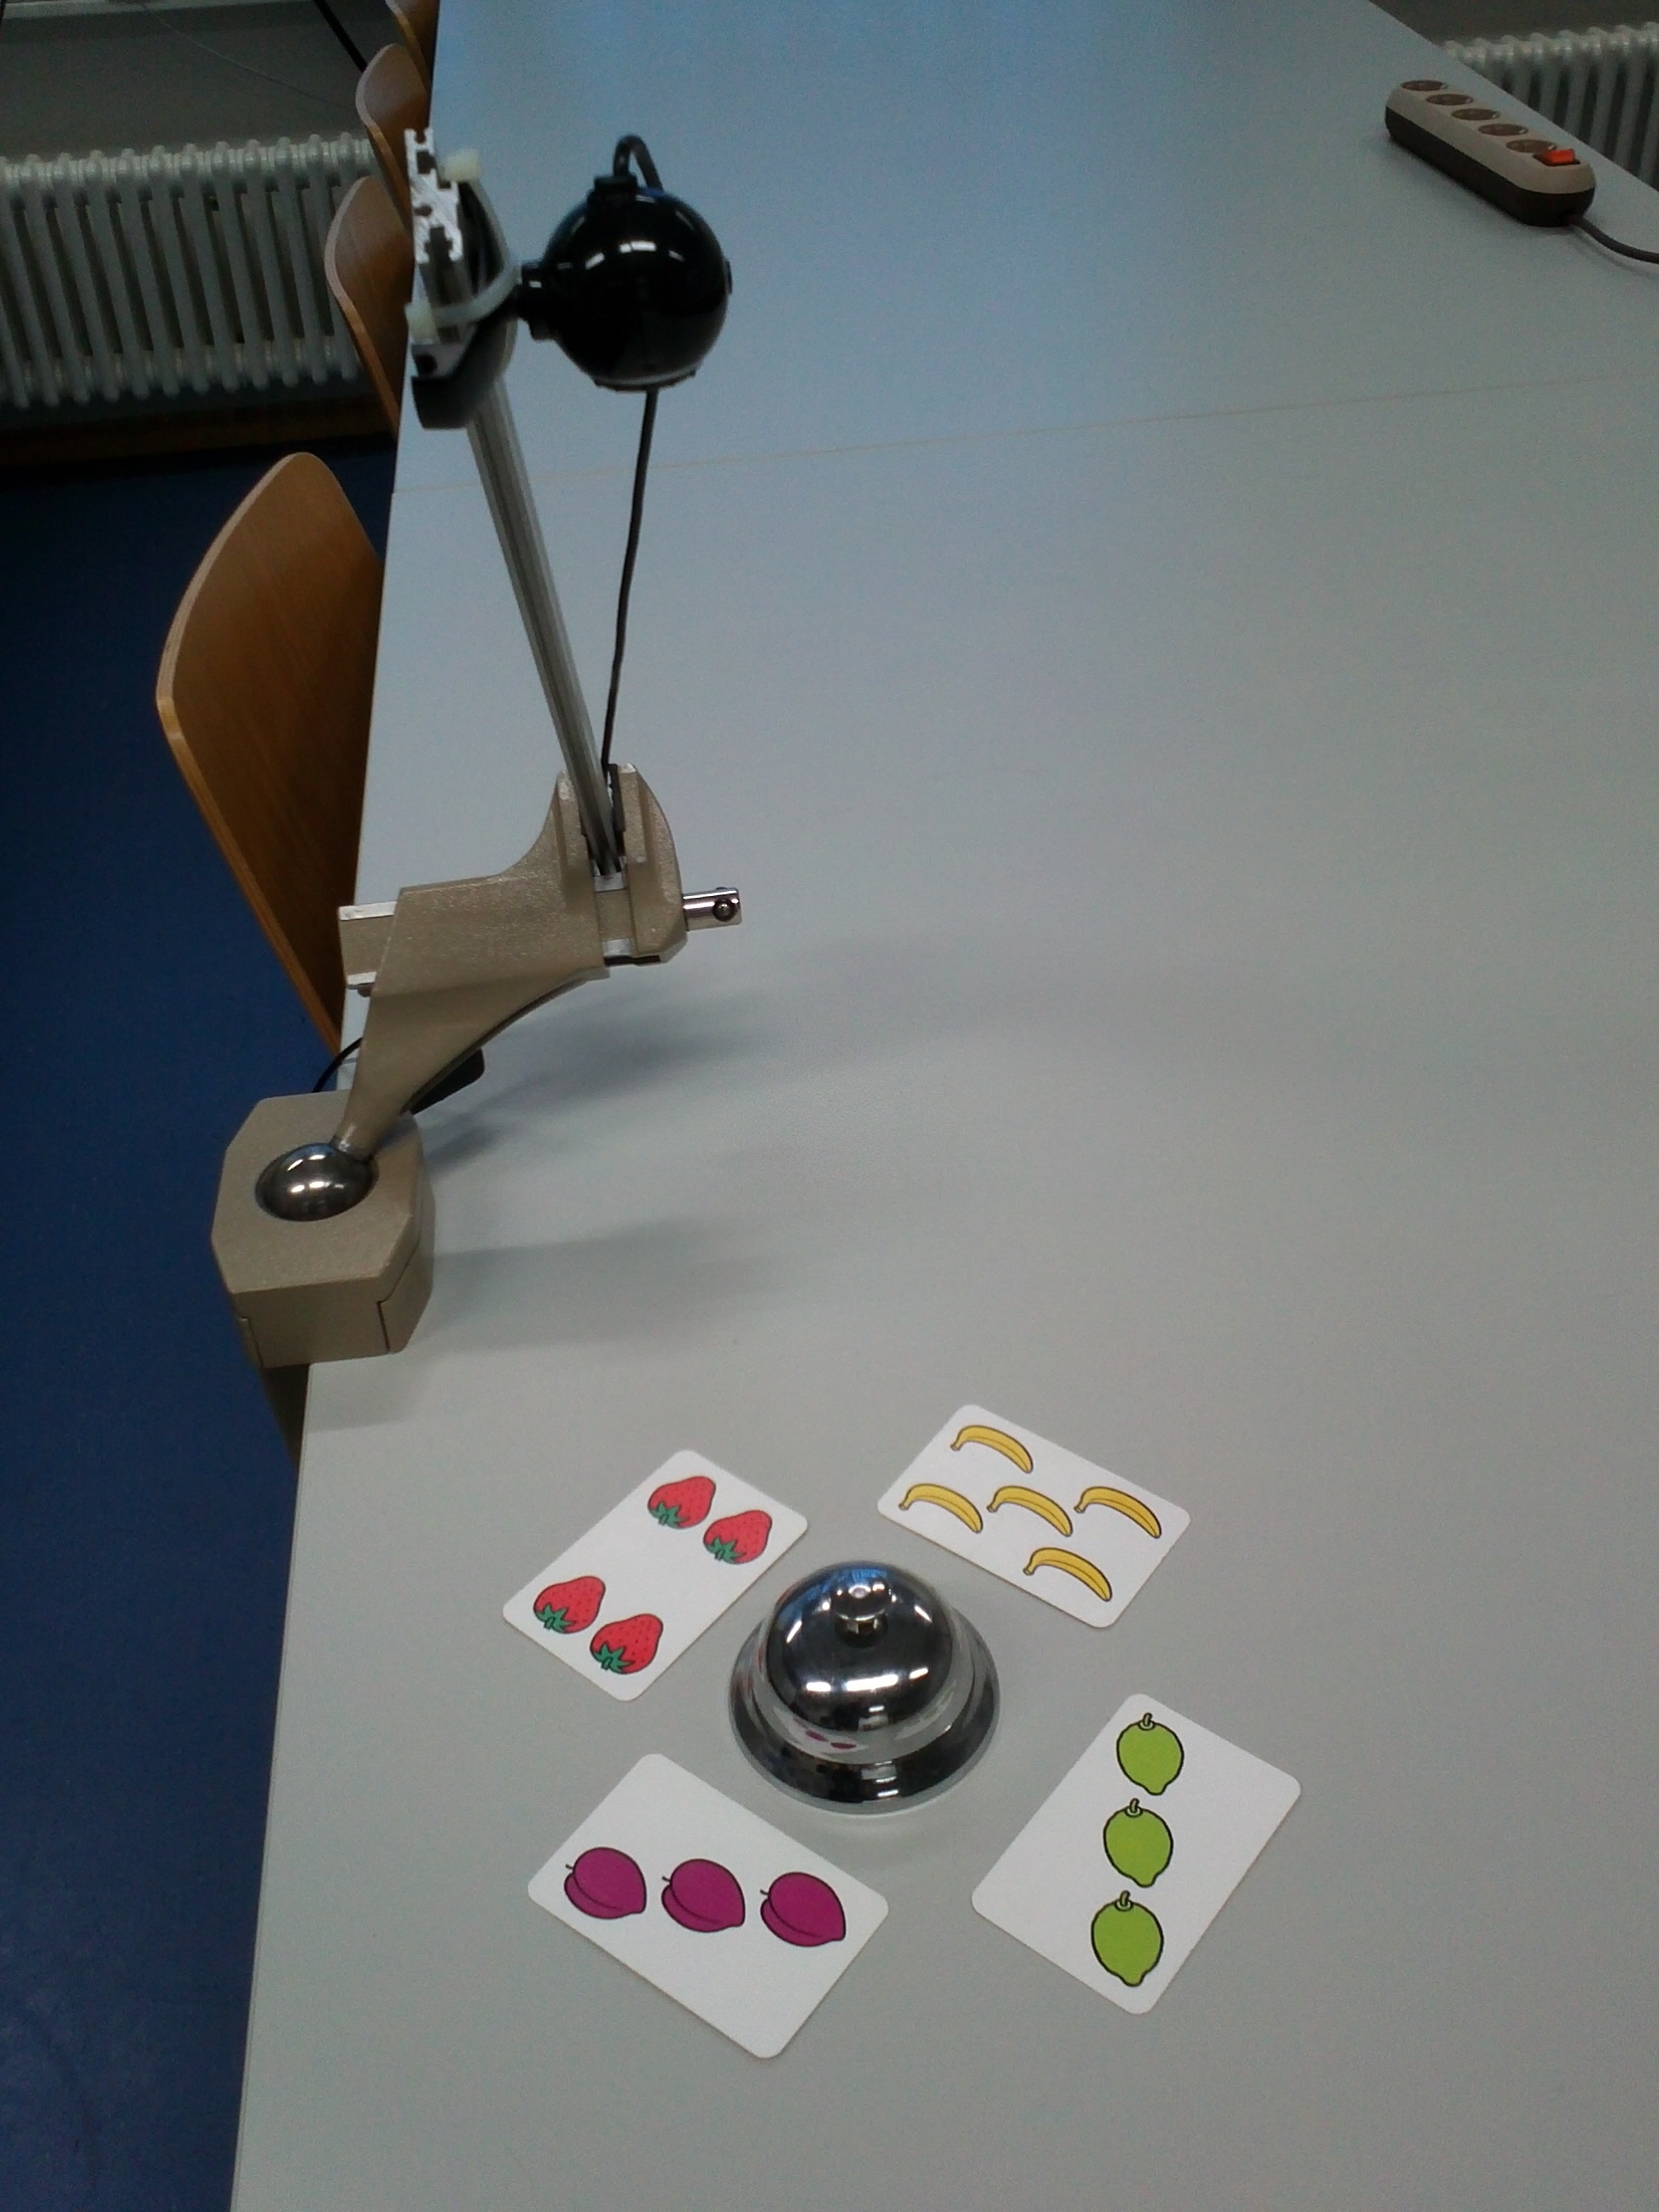
\includegraphics[width=7cm]{Abbildungen/KameraAufbau}
    \caption[Anlage]{Anlagenaufbau}
    \label{fig:Anlage}
\end{figure}

Der Spielaufbau entspricht dem original Halli Galli Aufbau mit vier Mitspielern. Abbildung~\ref{fig:Spielaufbau} zeigt die mittig positionierte Glocke, um die vier Ablagestabel der Spieler angeordnet sind.

%Abbildung Foto, wie die Karten liegen
\begin{figure}[h]
    \centering
    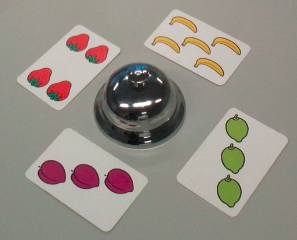
\includegraphics[width=6cm]{Abbildungen/Aufbau4}
    \caption[Spielaufbau]{Halli Galli - Spielaufbau mit vier Mitspielern}
    \label{fig:Spielaufbau}
\end{figure}

%Gibt es sonst noch was wichtiges zum Aufbau zu sagen?!?!?

% !TEX root = Calli.tex

\section{Programmstruktur / Methodik}
\label{sec:Programmstruktur}

Zum Lösen der Aufgabe wird die Programmiersprache \emph{Python 2.7} verwendet. In Form der Open-Source Library \emph{OpenCV} steht dazu eine leistungsstarke Bibliothek zur Bildverarbeitung zur Verfügung.
OpenCV selbst ist in C++ geschrieben, bietet jedoch entsprechende Python-Bindings an.


\subsection{Initialisierung}

Favorisiert wird eine extern angeschlossene Webcam angesprochen. Findet die Software keine Kamera, so greift sie auf die interne Kamera des Laptops zu. 
\begin{singlespace}
\lstset{language=Python}
\begin{lstlisting}[ ]
# try to use an external webcam if possible
cap = cv2.VideoCapture(1)
if not cap.isOpened():
    # use the internal cam
    cap = cv2.VideoCapture(0)
\end{lstlisting}
\end{singlespace}

\textbf{HSV-Raum}

Um die einzelnen Früchte sicher detektieren zu können, wird zuerst das Ausgangsbild in den HSV-Raum übertragen. Jede Farbe wird mit Hilfe des Farbwinkel (hue) auf dem Farbkreis (z.B. 0$^\circ$/360$^\circ$  für rot), der Farbsättigung (saturation) in Prozent (z.B. 0\% Neutralgrau) und des Hellwertes (value) in Prozent (z.B.100\% volle Helligkeit) definiert.
\begin{figure}[H]
    \centering
    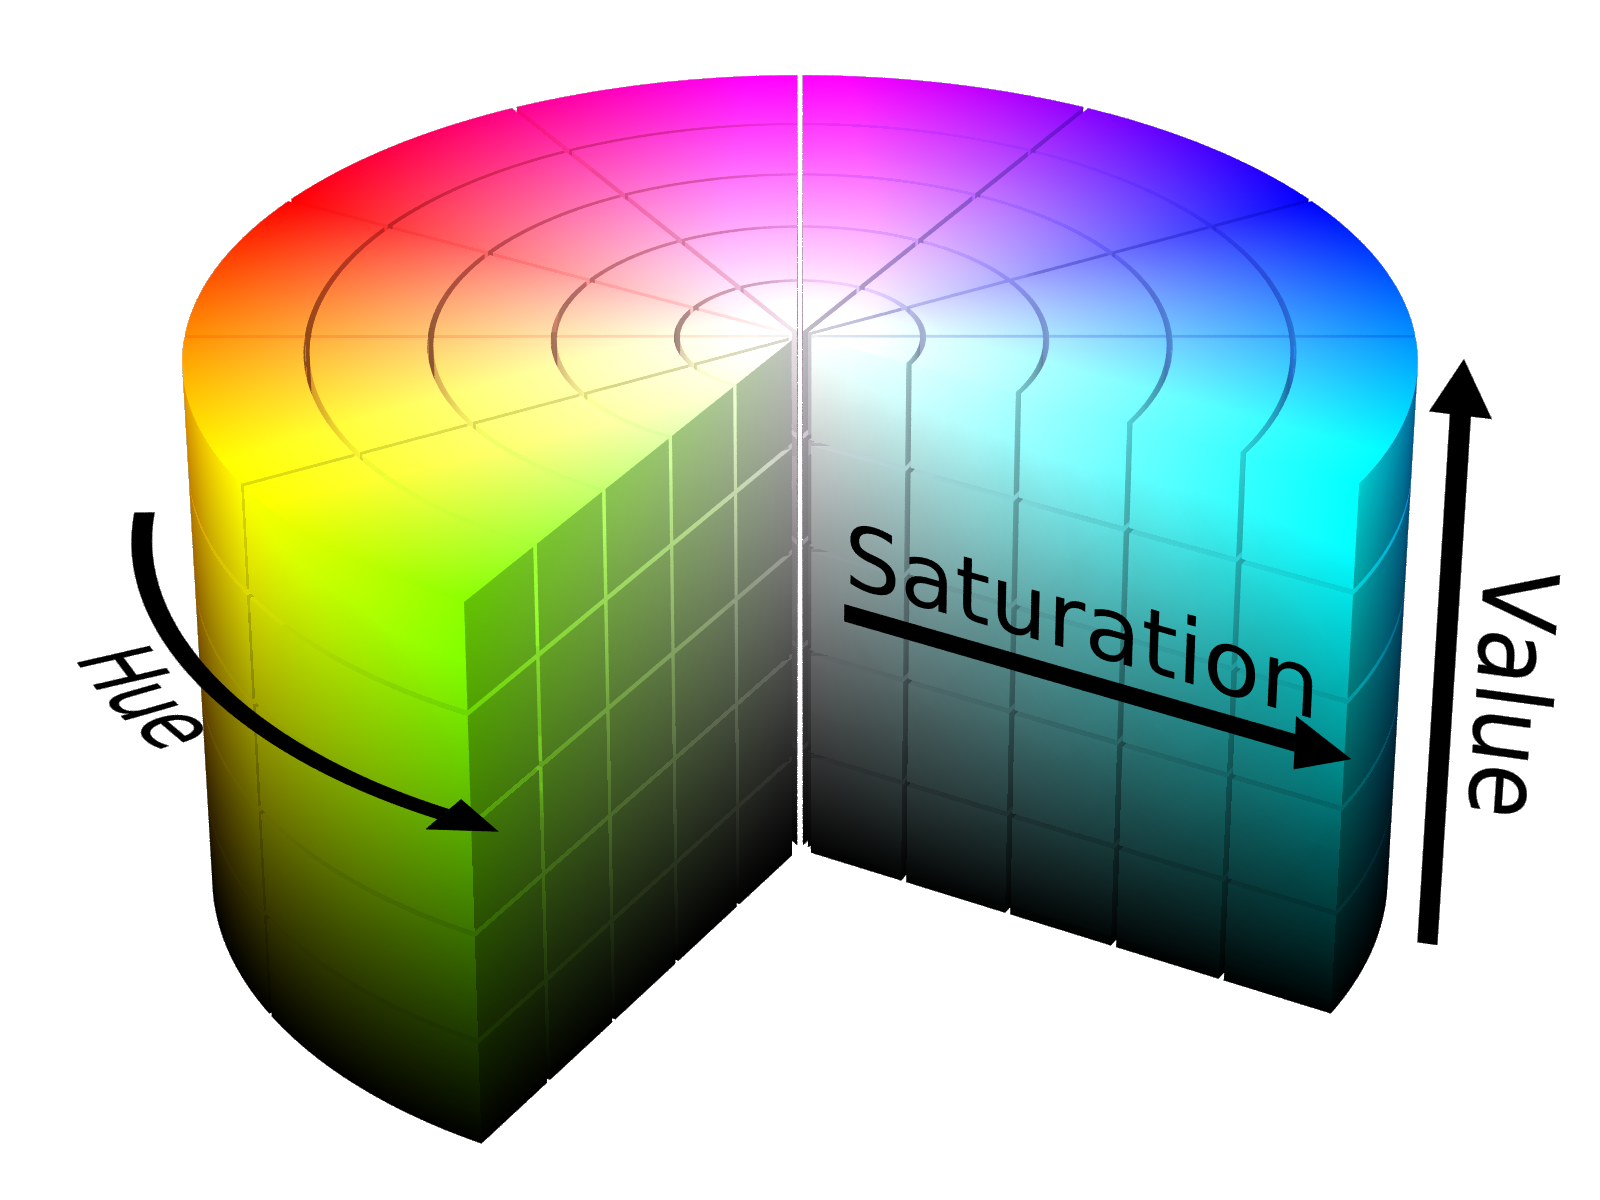
\includegraphics[width=0.4\textwidth]{Abbildungen/HSV_color}
    \caption[HSV]{HSV-Farbraum}
    \label{fig:HSV-Farbraum}
\end{figure}
\lstset{language=Python}
\begin{lstlisting}[]
    # read the frames
    _, frame = cap.read()
    # transform frame to HSV
    hsv = cv2.cvtColor(frame, cv2.COLOR_BGR2HSV)
\end{lstlisting}
In OpenCV wird der Farbwinkel mit 8~Bit im Bereich von 0 bis 179, die Farbsättigung mit vollen 8Bit von 0 bis 255 und die Helligkeit mit vollen 8~Bit von 0 bis 255 dargestellt.
Für die Farben der Früchte des Halli Galli Spiels ist der HSV-Raum fest definiert. Die Bereiche zur Filterung werden entsprechend darum festgelegt. 

\begin{itemize}
    \item Erdbeere - rot - HSV~(3, 73\%, 70\%)
    \item Pflaume - lila - HSV~(329, 68\%, 45\%)
    \item Limone - hellgrün - HSV~(93, 64\%, 57\%)
    \item Banane - gelb - HSV~(53, 72\%, 69\%)
\end{itemize}

Minimum - und Maximumwert für die Farbbereiche der Früchte können zur Kalibrierung über Schieberegler, darstellt in Abbildung ~\ref{fig:Regler}, eingestellt werden. Abhängig von der Beleuchtung und der verwendeten Kamera variieren diese, sodass eine Anpassung zum Beginn des Prozesses sinnvoll ist. 

\begin{figure}[H]
    \centering
    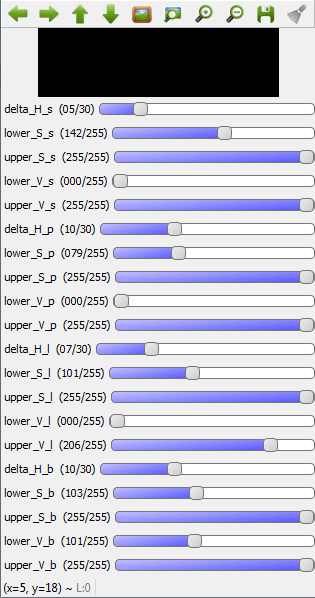
\includegraphics[width=0.4\textwidth]{Abbildungen/Regler02}
    \caption[Regler]{Schieberegler}
    \label{fig:Regler}
\end{figure}

\subsubsection{Schwellwertverfahren}

Mit Hilfe einer Segmentierung über ein Schwellwertverfahrens wird das Ausgangsbild für jede Fruchtsorte gefiltert und jeweils ein Binärbild erstellt. Im weiteren Bericht wird die Vorgehensweise jeweils an einem Fruchtbeispiel, welches besonders ist, erläutert. 

Da bei den Erdbeeren die Farbe Rot an den Grenzen des Farbwinkelwertes liegt, werden hier zwei Schwellwertoperationen durchgeführt und diese anschließen bitweise mit ODER zu einem verknüpft werden.
\lstset{language=Python}
\begin{lstlisting}[ ]
  # use Threshold for Strawberries
    thresh1_low = cv2.inRange(
        hsv,
        np.array((0, lower_s_s, lower_v_s)),
        np.array((0 + h_s, upper_s_s, upper_v_s)))
    thresh1_high = cv2.inRange(
        hsv,
        np.array((180 - h_s, lower_s_s, lower_v_s)),
        np.array((180, upper_s_s, upper_v_s)))
    thresh1 = cv2.bitwise_or(thresh1_low, thresh1_high)
\end{lstlisting}

\subsubsection{Filter}

Für jede Frucht wird das Ausgangsbild mit einem Closing - Operator und einem Opening - Operator gefiltert. Während durch das Closing dunkle Störungen im Bild unterdrückt werden, vermindert das Opening lokale Störungen durch helle Bildpunkte.  \\
\lstset{language=Python}
\begin{lstlisting}[ ]
    # Opening
    thresh3 = cv2.morphologyEx(thresh3, cv2.MORPH_OPEN, kernel)
    # Closing
    thresh3 = cv2.morphologyEx(thresh3, cv2.MORPH_CLOSE, kernel)
\end{lstlisting}

\subsection{Konturerkennung}
%beschreibung der Konturerkennung vllt. an Hand der Skrips
Nach der Vereinzelung jeder Frucht werden die gefundenen Bildpunkte zu Segmenten zusammengefasst und mit einer Kontur umgeben. 

\lstset{language=Python}
\begin{lstlisting}[ ]
    strawberry_contours, strawberry_hierarchy = cv2.findContours(
        thresh1,
        cv2.RETR_LIST,
        cv2.CHAIN_APPROX_SIMPLE)
\end{lstlisting}

\subsection{Formsegmentierung}

Wenn alle Pixel in den Farben der Früchte entdeckt und segmentiert sind, ist es notwendig die Form der gefundenen Segmente zu untersuchen. Dazu werden für jede Frucht verschiedene geometrische Verhältnisse betrachtet.
\begin{itemize}
    \item Größe der Fläche
    \item Seitenverhältnis des kleinst - möglich umgebenden Rechteckes
    \item Verhältnis Größe der Fläche zu Größe des kleinst - möglich umgebenden Rechteckes
\end{itemize}
Im Fall der Bananen muss zusätzlich die Ausrichtung des umschließenden Rechtecks überprüft werden, um den zutreffenden einstellbaren Filterbereich zu verkleinern. 
Zur Justierung der Parameter werden die Werte an den Konturen ausgegeben.
\lstset{language=Python}
\begin{lstlisting}[ ]
    # Find Bananas
    bananas = []
    for cnt in banana_contours:
        banana_area = cv2.contourArea(cnt)
        (x_c, y_c), radius = cv2.minEnclosingCircle(cnt)
        center = int(x_c), int(y_c)
        radius = int(radius)
        rect = cv2.minAreaRect(cnt)
        pos, size, theta = rect
        box = cv2.cv.BoxPoints(rect)
        box = np.int0(box)
        x, y = pos
        w, h = size
        if 300 < banana_area < 900:
            if h < w:
                w, h = h, w
            if 2.0 < h / w < 3.9:
                area_rate = w * h / banana_area  # 1.7
                if 1.2 < area_rate < 2.9:
                    bananas.append(cnt)
                    # draw_str(
                    #   frame,
                    #   (int(x)+radius, int(y)),
                    #   str(h/w))
                    # draw_str(
                    #   frame,
                    #   (int(x)+radius, int(y)+24),
                    #   str(banana_area))
                    # draw_str(
                    #   frame,
                    #   (int(x)+radius, int(y)+12),
                    #   str(area_rate))
                    # cv2.drawContours(frame,[box],0,(0,255,0),2)
\end{lstlisting}
\begin{figure}[H]
    \centering
    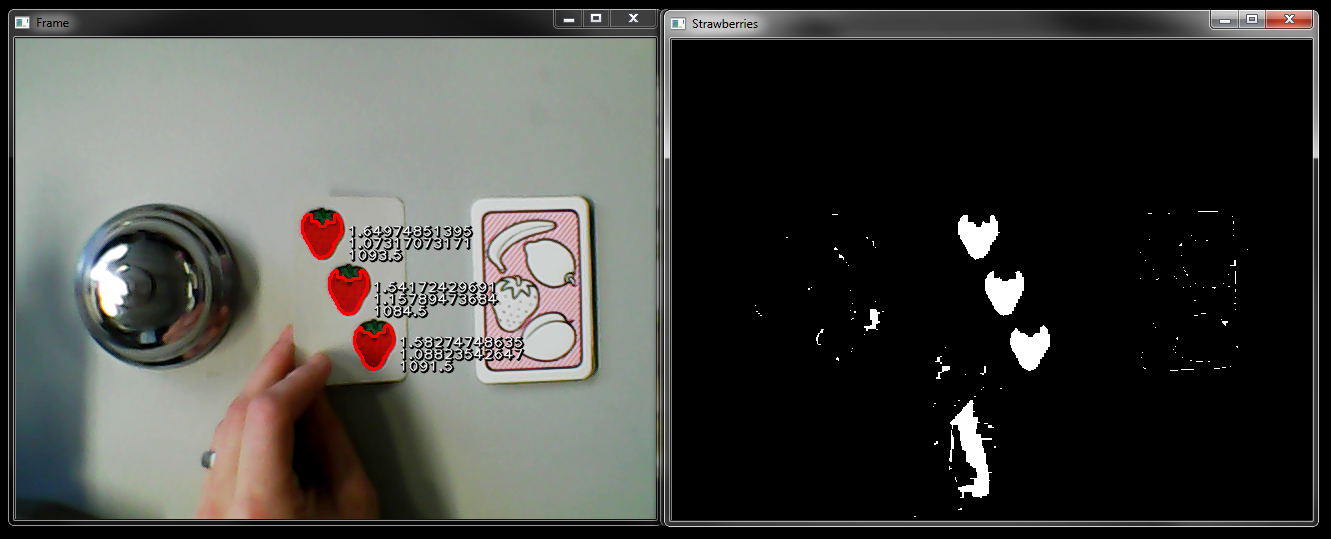
\includegraphics[width=\textwidth]{Abbildungen/Erdbeeren03}
    \caption[ ]{Erkannte Erdbeeren mit Wertausgabe}
    \label{fig:Erdbeeren03}
\end{figure}
\begin{figure}[H]
    \centering
    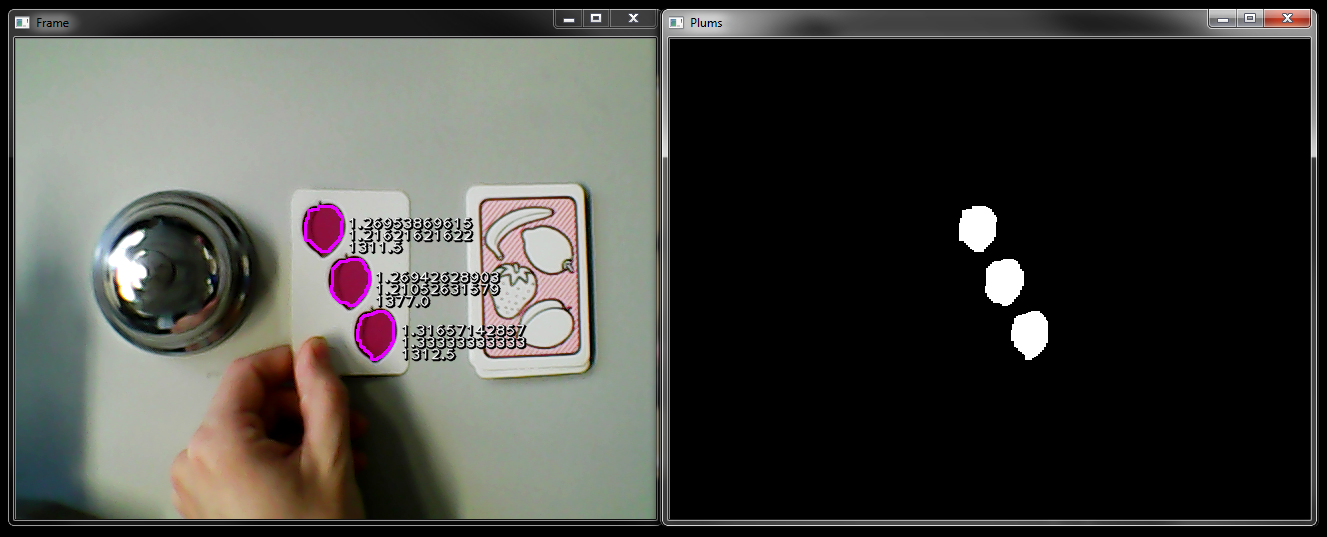
\includegraphics[width=\textwidth]{Abbildungen/Pflaumen03}
    \caption[ ]{Erkannte Pflaumen mit Wertausgabe}
    \label{fig:Pflaumen03}
\end{figure}
\begin{figure}[H]
    \centering
    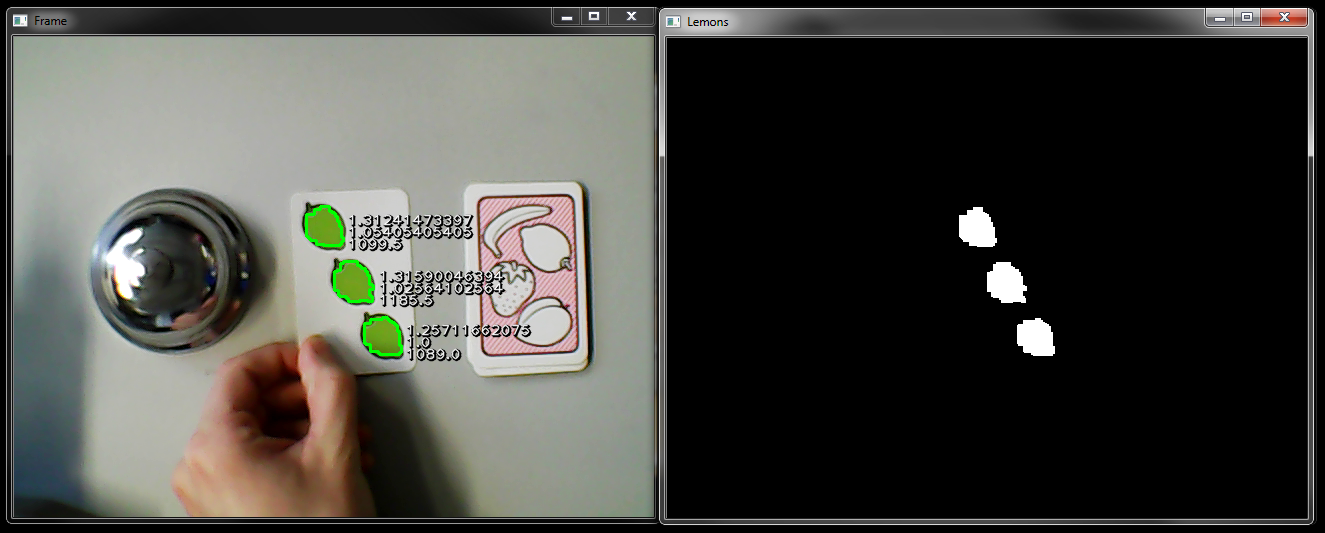
\includegraphics[width=\textwidth]{Abbildungen/Limetten03}
    \caption[ ]{Erkannte Limonen mit Wertausgabe}
    \label{fig:Limetten03}
\end{figure}
\begin{figure}[H]
    \centering
    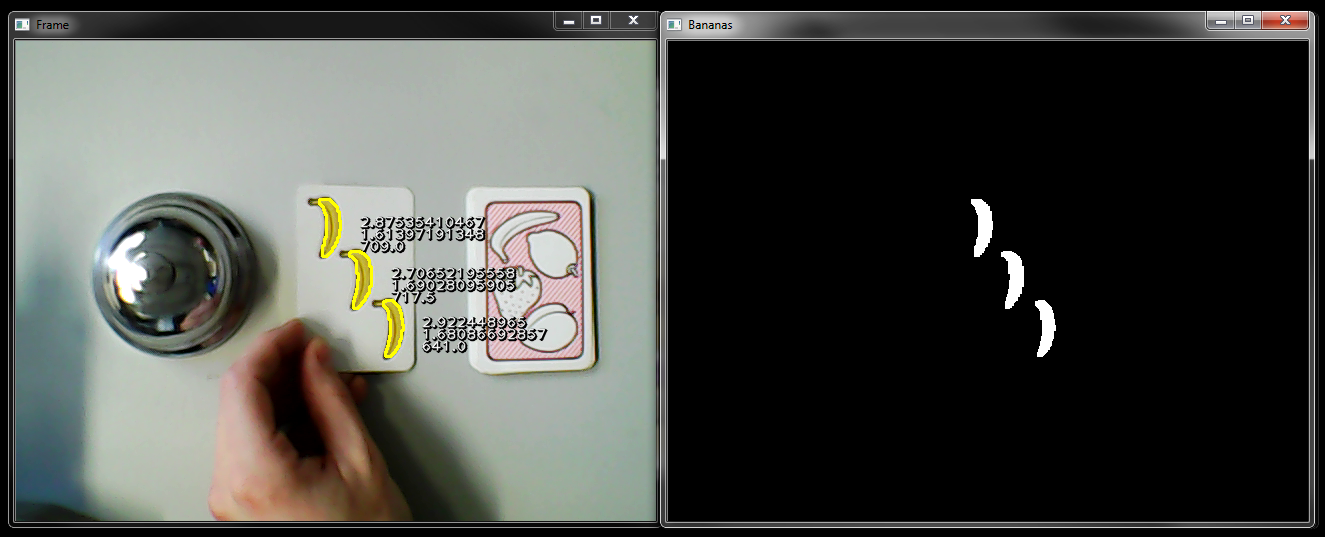
\includegraphics[width=\textwidth]{Abbildungen/Bananen03}
    \caption[ ]{Erkannte Bananen mit Wertausgabe}
    \label{fig:Bananen03}
\end{figure}

\subsection{Auswertung}

Zur Auswertung werden die gefunden Früchte automatisch gezählt. Werden genau fünf Früchte einer Sorte gefunden, signalisiert ein Schriftzug auf dem Bildschirm, welche Frucht gefunden wurde und dass die Glocke geläutet werden muss. \textbf{Auf die Glocke, fertig los!}

\lstset{language=Python}
\begin{lstlisting}[ ]
   cv2.namedWindow('Frame')
    cv2.drawContours(frame, strawberries, -1, (0, 0, 255), 2)
    cv2.drawContours(frame, plums, -1, (255, 0, 230), 2)
    cv2.drawContours(frame, lemons, -1, (0, 255, 0), 2)
    cv2.drawContours(frame, bananas, -1, (0, 255, 255), 2)
    if len(strawberries) == 5:
        # print "Strawberries!"
        draw_str(frame, (20, 20), "Strawberries!!!!!")
    if len(plums) == 5:
        # print "Plums!"
        draw_str(frame, (20, 40), "Plums!!!!!")
    if len(lemons) == 5:
        # print "Lemons!"
        draw_str(frame, (20, 60), "Lemons!!!!!")
    if len(bananas) == 5:
        # print "Bananas!"
        draw_str(frame, (20, 80), "Bananas!!!!!")
    cv2.imshow('Frame', frame)
\end{lstlisting}




% !TEX root = Calli.tex
% Kapitelvorlage

\section{Anleitung}
\label{sec:Anleitung}

\subsection{Anwendung mit Kamera-Stream}
Um das Programm mit dem geringsten Aufwand ausführen zu können, wurde mit dem \emph{PyInstaller} aus dem Python-Programm eine exe-Anwendung erstellt. Diese Version ist auf eine Web-Cam in 40cm über der Spielfläche bei indirekter Beleuchtung eingestellt. 


\subsection{Konsolenanwendung für Bilder}
Für Demonstrationszwecke wurde eine Variante als Konsolenanwendung erstellt, um das Programm ohne Kamera mit Beispielbildern zu testen. 
An die Anwendung wird mit dem Kürzel \lstinline{-i} die Bilddatei angehängt.
 
Wahlweise können mit Optionskürzeln zusätzliche Informationen angezeit werden:
\begin{itemize}
\item \lstinline{-c} zeigt die Kontur der umschließenden Rechtecke an 
\item \lstinline{-o} zeigt die Textausgabe der Werte in der Formsegmentierung an
\end{itemize}
\begin{lstlisting}[ ]
cd <programdir>
Calli-Cv-Pictures.exe -i Testbild01.PNG -c -o
\end{lstlisting}

% !TEX root = Calli.tex
% Kapitelvorlage

\section{OpenCV - Python}
\label{sec:OpenCV}

\subsection{Quellcode der Programmversion mit Kamera-Stream:}
\lstset{language=Python}
\lstinputlisting{../calli-cv.py}

\subsection{Quellcode des Programms mit Bildern als Konsolenversion:}
\lstset{language=Python}
\lstinputlisting{../calli-cv-Pictures.py}


% !TEX root = Frontkollisionsassistenzsysteme.tex
\begin{thebibliography}{sotief}
\bibliographystyle{dinat} % DIN-Stil des Literaturverzeichnisses

\bibitem[Bie 13]{Bie 13}
Biegert, Marco; Funk, Andreas:
\newblock {\em B~\&~F Manufacture Verwaltungs-GmbH} %Register-Nr.:~HRB~729102,}
\newblock \\URL: http://www.qlocktwo.com/news.php?lang=de (Stand: 02.12.2013)

\bibitem[Con 13]{Con 13}
Conway, John Horton:
\newblock {\em Conways Spiel des Lebens}
\newblock \\URL: http://de.wikipedia.org/wiki/Conways\_Spiel\_des\_Lebens (Stand: 02.12.2013)

\end{thebibliography}



\end{document}
